\chapter{Identical Particles}

In classical mechanics and the macroscopic systems, one can distinguish any particle from another by looking at its properties. However, particles in quantum mechanical systems cannot be distinguished by their size, shape or location as they lack these properties. To demonstrate this consider a collision event between two particles of the same kind and draw a box around the collision point as demonstrated in Figure (\ref{fig:identicalcollision}).

\begin{figure}[h!]
    \centering
    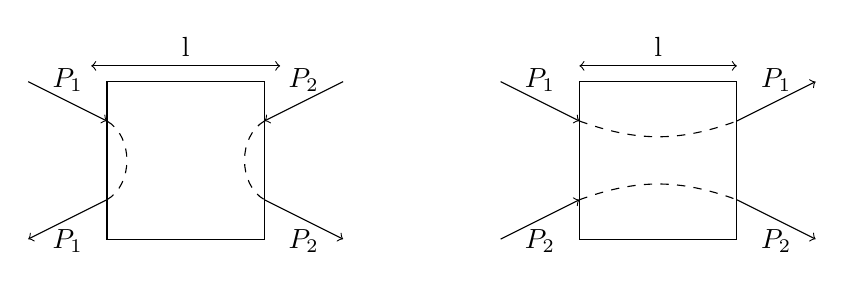
\begin{tikzpicture}
       % First diagram on the left
        \draw[->] (-2,1) -- (-1,0.5) node[midway, above] {$P_1$};
        \draw[->] (-1,-0.5) -- (-2,-1)   node[midway, below] {$P_1$};
        \draw[->] (2,1) -- (1,0.5)  node[midway, above] {$P_2$};
        \draw[->] (1,-0.5) -- (2,-1) node[midway, below] {$P_2$};
        
        % Curved dashed lines inside the square
        \draw[dashed] (-1,-0.5) to[out=30,in=-30] (-1,0.5);
        \draw[dashed] (1,0.5) to[out=210, in=150] (1,-0.5);
        
        \draw (-1,1) -- (1,1) -- (1,-1) -- (-1,-1) -- cycle;
        
        \draw[<->] (-1.2,1.2) -- (1.2,1.2) node[midway, above] {l};
        
        % Second diagram on the right (same as the left)
        \draw[->] (4,1) -- (5,0.5) node[midway, above] {$P_1$};
        \draw[->] (4,-1) -- (5,-0.5) node[midway, below] {$P_2$};
        \draw[->] (7,0.5) -- (8,1) node[midway, above] {$P_1$};
        \draw[->] (7,-0.5) -- (8,-1) node[midway, below] {$P_2$};
        
        % Curved dashed lines inside the square (curved outward)
        \draw[dashed] (5,0.5) to[out=-20,in=200] (7,0.5);
        \draw[dashed] (5,-0.5) to[out=20,in=-200] (7,-0.5);
        
        
        
        \draw (5,1) -- (7,1) -- (7,-1) -- (5,-1) -- cycle;
        
        \draw[<->] (5,1.2) -- (7,1.2) node[midway, above] {l};
        
    \end{tikzpicture}
    \caption{Two possible collision events between particles of the same kind.}
    \label{fig:identicalcollision}
\end{figure}

If the size of the box is at the order of magnitude as the uncertainty in their positions, then we cannot know which of the two processes took place. In that case, the particles are said to be \textbf{indistinguishable}. \\
Now, consider a wavefunction of two particles $\psi(x_1,x_2)$ where $x_1$ and $x_2$ are composite position-spin coordinates: $x_i = (\v{r}_i,\sigma_i)$. If the two particles are indistinct, then the expectation values cannot change under an exchange of $x_1$ and $x_2$. Howver, the wavefunction itself may not be invariant. Consider the expectation value of a Hamiltonian. 
\begin{equation}
    \expval{\hat{H}} = \int dx_1dx_2\psi^*(x_1,x_2)\hat{H}(x_1,x_2)\psi(x_1,x_2) = E\int dx_1dx_2\abs{\psi(x_1,x_2)}^2
\end{equation}
Now, if we exchange the two particles, the expectation value should be the same. Moreover, since the Hamiltonian is symmetric, it will give the same eigenvalue. 
\begin{equation}
    \expval{\hat{H}} = \int dx_2dx_1\psi^*(x_2,x_1)\hat{H}(x_2,x_1)\psi(x_1,x_2)=E\int dx_2dx_1\abs{\psi(x_2,x_1)}^2
\end{equation}
Since $dx_1$ and $dx_2$ commute in the integration measure, this equality implies
\begin{equation}
    \abs{\psi(x_1,x_2)}^2 = \abs{\psi(x_2,x_1)}^2.
\end{equation}
From this equality, we can see that the two wavefunctions differ only by a phase factor.
\begin{equation}
    \psi(x_2,x_1)=e^{i\alpha}\psi(x_1,x_2)
\end{equation}
Note that for such a two-particle system, we have to obtain the original wavefunction upon doing another exchange. Then,
\begin{equation}
    \psi(x_1,x_2) = (e^{i\alpha})^2\psi(x_1,x_2)
\end{equation}
This means that there are only two possible values for $\alpha$: $\alpha=0$ and $\alpha=\pi$. These correspond to two different types of particles:
\begin{itemize}
    \item[i)] \textbf{Bosons:} Symmetric wavefunctions $\psi(x_1,x_2)=\psi(x_2,x_1)$
    \item[ii)] \textbf{Fermions}: Antisymmetric wavefunctions $\psi(x_1,x_2)=-\psi(x_2,x_1)$
\end{itemize}
\section{Bosons}
    Imagine a Helium atom with one-particle states $\phi_i(\v{r})$. Now, consider a wavefunction describing two non-interacting Helium atoms together. Assuming that $\{\phi_i(\v{r})\}$ form an orthonormal basis set, we can ansatz the wavefunction of the whole system as
    \begin{equation}
        \psi(\v{r}_1,\v{r}_2)=\phi_i(\v{r}_1)\phi_j(\v{r}_2).
    \end{equation}
    Here, we exclude the spins as the Helium atom has spin zero. This wavefunction is neither symmetric nor antisymmetric. To symmetrize it let us add a term with the particles switched.
    \begin{equation}
        \psi(\v{r}_1,\v{r}_2)=\frac{1}{\sqrt{2}}(\phi_i(\v{r}_1)\phi_j(\v{r}_2)+\phi_i(\v{r}_2)\phi_j(\v{r}_1))
    \end{equation}
    We can furhter consider a three-particle state. 
    \begin{equation}
        \psi(\v{r}_1,\v{r}_2,\v{r}_3) = \frac{1}{\sqrt{3!}}(\phi_i(\v{r}_1)\phi_j(\v{r}_2)\phi_k(\v{r}_3)+\phi_i(\v{r}_1)\phi_j(\v{r}_3)\phi_k(\v{r}_2)+...)
    \end{equation}
    For bosons, we can have multiple particles occupying the same position/orbit. This gives
    \begin{equation}
        \psi(\v{r}_1,\v{r}_2)=\phi_i(\v{r}_1)\phi_i(\v{r}_1) \implies E = 2\varepsilon_i.
    \end{equation}
    This allows us to label the wavefunctions only by the occupation numbers: How many particles occupy a single state.
    \begin{equation}
        \psi = \ket{n_1n_2n_3...}
    \end{equation}
    \begin{problem}{Find the total energy of five harmonic oscillators in a many-particle state given by the wavefunction 
    \begin{equation}
        \psi = \ket{1021}.
    \end{equation}
    }
    Recall that the energy of the harmonic oscillator was
    \begin{equation}
        \varepsilon_n = \lrp{n+\frac{1}{2}}\hbar\omega.
    \end{equation}
    Then, $\varepsilon_0=\hbar\omega/2$, $\varepsilon_1=0$ $\varepsilon_2=5\hbar\omega/2$, and $\varepsilon_3 = 7\hbar\omega/2$. This gives us
    \begin{equation}
        E = \frac{\hbar\omega}{2} + \frac{5\hbar\omega}{2} + \frac{7\hbar\omega}{2} = 9\hbar\omega.
    \end{equation}
    \end{problem}
\section{Fermions}
    For fermions, the wavefunction is antisymmetric. Let us construct an antisymmetric wavefunction for two particles as we did in a similar way before. 
    \begin{equation}
        \psi(\v{r}_1,\v{r}_2) = \frac{1}{\sqrt{2}}(\phi_i(\v{r}_1)\phi_j(\v{r}_2)-\phi_i(\v{r}_2)\phi_j(\v{r}_1))
    \end{equation}
    Note that, this construction looks like a determinant.
    \begin{equation}
        \psi(\v{r}_1,\v{r}_2)=\frac{1}{\sqrt{2}}\begin{vmatrix}
            \phi_i(\v{r}_1) & \phi_j(\v{r}_1) \\ 
            \phi_i(\v{r}_2) & \phi_j(\v{r}_2)
        \end{vmatrix}
    \end{equation}
    For three particles, we get
    \begin{equation}
        \psi(\v{r}_1,\v{r}_2,\v{r}_3) = \frac{1}{\sqrt{6}}\begin{vmatrix}
            \phi_i(\v{r}_1) & \phi_j(\v{r}_1) & \phi_k(\v{r}_1) \\ 
            \phi_i(\v{r}_2) & \phi_j(\v{r}_2) & \phi_k(\v{r}_2) \\ 
            \phi_i(\v{r}_3) & \phi_j(\v{r}_3) & \phi_k(\v{r}_3)
        \end{vmatrix}
    \end{equation}
    Unlike bosons, if two fermions occupy the same state, then the determinant and thus the wavefunction becomes zero. This means that the probability of multiple particles occupying the same state is zero. This is the \textbf{Pauli exclusion principle}. We can still label the wavefunction by the occupation numbers but these numbers can only be 0 or 1. \\
    With this construction of wavefunction, we can generalise the energy of both the fermions and bosons as
    \begin{equation}
        E = \sum_in_i\varepsilon_i \hspace{0.5cm}\mathrm{where}\hspace{0.5cm}\sum_in_i=N.
    \end{equation}
\newpage
\section{Partition Function}
    Let us now imagine a two-particle system with three energy levels. Considering that the particles are bosons, all possible two-particle states are: 
    \begin{figure}[h!]
        \centering
        \resizebox{0.9\textwidth}{!}{%
        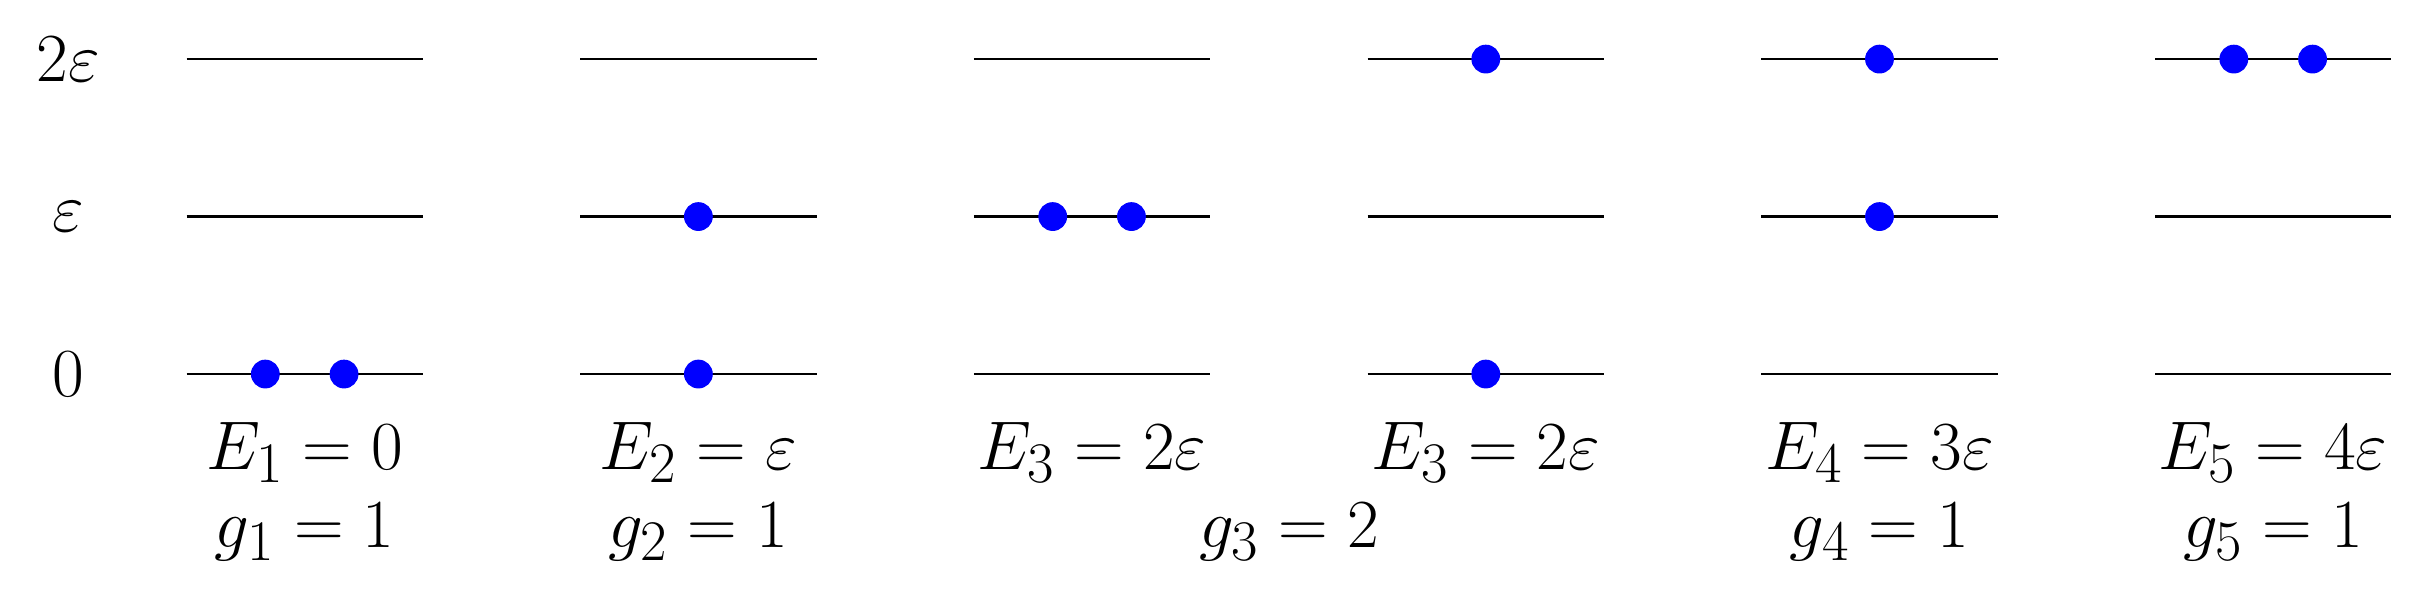
\begin{tikzpicture}
            \draw[black,thick] (0,0) -- (3,0);
            \draw[black,thick] (5,0) -- (8,0);
            \draw[black,thick] (10,0) -- (13,0);
            \draw[black,thick] (15,0) -- (18,0);
            \draw[black,thick] (20,0) -- (23,0);
            \draw[black,thick] (25,0) -- (28,0);
            \draw[black,thick] (0,2) -- (3,2);
            \draw[black,thick] (5,2) -- (8,2);
            \draw[black,thick] (10,2) -- (13,2);
            \draw[black,thick] (15,2) -- (18,2);
            \draw[black,thick] (20,2) -- (23,2);
            \draw[black,thick] (25,2) -- (28,2);
            \draw[black,thick] (0,4) -- (3,4);
            \draw[black,thick] (5,4) -- (8,4);
            \draw[black,thick] (10,4) -- (13,4);
            \draw[black,thick] (15,4) -- (18,4);
            \draw[black,thick] (20,4) -- (23,4);
            \draw[black,thick] (25,4) -- (28,4);
            \node[black,thick] at(-1.5,0) {\Huge$0$};
            \node[black,thick] at(-1.5,2) {\Huge$\varepsilon$};
            \node[black,thick] at(-1.5,4) {\Huge$2\varepsilon$};
            \node[black,thick] at(1.5, -1) {\Huge$E_1 = 0$};
            \node[black,thick] at(1.5, -2) {\Huge$g_1 = 1$};
            \node[black,thick] at(6.5, -1) {\Huge$E_2 = \varepsilon$};
            \node[black,thick] at(6.5, -2) {\Huge$g_2 = 1$};
            \node[black,thick] at(11.5, -1) {\Huge$E_3 = 2\varepsilon$};
            \node[black,thick] at(16.5, -1) {\Huge$E_3=2\varepsilon$};
            \node[black,thick] at(14, -2) {\Huge$g_3 = 2$};
            \node[black,thick] at(21.5, -1) {\Huge$E_4 = 3\varepsilon$};
            \node[black,thick] at(21.5, -2) {\Huge$g_4 = 1$};
            \node[black,thick] at(26.5, -1) {\Huge$E_5 = 4\varepsilon$};
            \node[black,thick] at(26.5, -2) {\Huge$g_5 = 1$};
            \filldraw [blue] (1,0) circle (5pt);
            \filldraw [blue] (2,0) circle (5pt);
            \filldraw [blue] (11,2) circle (5pt);
            \filldraw [blue] (12,2) circle (5pt);
            \filldraw [blue] (26,4) circle (5pt);
            \filldraw [blue] (27,4) circle (5pt); 
            \filldraw [blue] (6.5, 0) circle (5pt);
            \filldraw [blue] (6.5,2) circle (5pt);
            \filldraw [blue] (16.5, 0) circle (5pt);
            \filldraw [blue] (16.5,4) circle (5pt);
            \filldraw [blue] (21.5, 2) circle (5pt);
            \filldraw [blue] (21.5, 4) circle (5pt);
        \end{tikzpicture}
        }
        \caption{Energy levels and occupations of a two-boson system with three energy levels.}
        \label{fig:bosonenergy}
    \end{figure}
    In this case, the partition function is given as
    \begin{equation}
        Z = \sum g_ne^{-\beta E_n} = 1 + e^{-\beta\varepsilon} + 2e^{-2\beta\varepsilon} + e^{-3\beta\varepsilon} + e^{-4\beta\varepsilon}.
    \end{equation}
    Similarly, if one considers fermions, the double occupation of energy levels is not allowed and we get the following.
    \begin{figure}[h!]
        \centering
        \resizebox{0.45\textwidth}{!}{%
        \begin{tikzpicture}
            \draw[black,thick] (0,0) -- (3,0);
            \draw[black,thick] (5,0) -- (8,0);
            \draw[black,thick] (10,0) -- (13,0);
            \draw[black,thick] (0,2) -- (3,2);
            \draw[black,thick] (5,2) -- (8,2);
            \draw[black,thick] (10,2) -- (13,2);
            \draw[black,thick] (0,4) -- (3,4);
            \draw[black,thick] (5,4) -- (8,4);
            \draw[black,thick] (10,4) -- (13,4);
            \node[black,thick] at(-1.5,0) {\Huge$0$};
            \node[black,thick] at(-1.5,2) {\Huge$\varepsilon$};
            \node[black,thick] at(-1.5,4) {\Huge$2\varepsilon$};
            \filldraw [blue] (1.5, 0) circle (5pt);
            \filldraw [blue] (1.5,2) circle (5pt);
            \filldraw [blue] (6.5,0) circle (5pt);
            \filldraw [blue] (6.5,4) circle (5pt);
            \filldraw [blue] (11.5, 2) circle (5pt);
            \filldraw [blue] (11.5,4) circle (5pt);
        \end{tikzpicture}
        }
        \caption{Energy levels and occupations of a two-fermion system with three energy levels}
        \label{fig:fermionenergy}
    \end{figure}
    
    In this case, the partiton function is
    \begin{equation}
        Z = e^{-\beta\varepsilon} + e^{-2\beta\varepsilon} + e^{-3\beta\varepsilon}.
    \end{equation}
    Now consider a system consisting of two distinguishable particles. 
    \begin{figure}[h!]
        \centering
        \resizebox{0.8\textwidth}{!}{%
        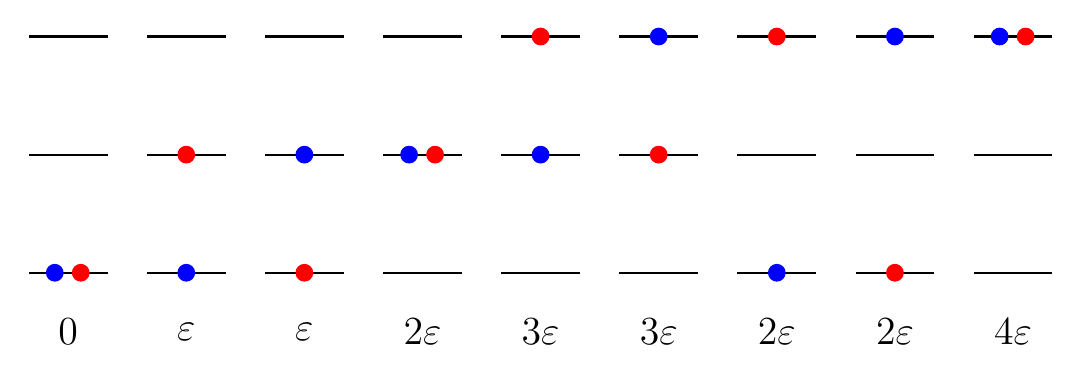
\begin{tikzpicture}
            \draw[black,thick] (0,0)--(1,0);
            \draw[black,thick] (1.5,0)--(2.5,0);
            \draw[black,thick] (3,0) -- (4,0);
            \draw[black,thick] (4.5,0) -- (5.5,0);
            \draw[black,thick] (6,0) -- (7,0);
            \draw[black,thick] (7.5, 0) -- (8.5,0);
            \draw[black,thick] (9,0) -- (10,0);
            \draw[black, thick] (10.5,0) -- (11.5,0);
            \draw[black,thick] (12,0) -- (13,0);

            \draw[black,thick] (0,1.5)--(1,1.5);
            \draw[black,thick] (1.5,1.5)--(2.5,1.5);
            \draw[black,thick] (3,1.5) -- (4,1.5);
            \draw[black,thick] (4.5,1.5) -- (5.5,1.5);
            \draw[black,thick] (6,1.5) -- (7,1.5);
            \draw[black,thick] (7.5, 1.5) -- (8.5,1.5);
            \draw[black,thick] (9,1.5) -- (10,1.5);
            \draw[black, thick] (10.5,1.5) -- (11.5,1.5);
            \draw[black,thick] (12,1.5) -- (13,1.5);

            \draw[black,thick] (0,3)--(1,3);
            \draw[black,thick] (1.5,3)--(2.5,3);
            \draw[black,thick] (3,3) -- (4,3);
            \draw[black,thick] (4.5,3) -- (5.5,3);
            \draw[black,thick] (6,3) -- (7,3);
            \draw[black,thick] (7.5, 3) -- (8.5,3);
            \draw[black,thick] (9,3) -- (10,3);
            \draw[black, thick] (10.5,3) -- (11.5,3);
            \draw[black,thick] (12,3) -- (13,3);

            \node[black, thick] at(0.5, -0.75) {\Large$0$};
            \node[black,thick] at(2, -0.75) {\Large$\varepsilon$};
            \node[black,thick] at(3.5, -0.75) {\Large$\varepsilon$};
            \node[black,thick] at(5, -0.75) {\Large$2\varepsilon$};
            \node[black,thick] at(6.5, -0.75) {\Large$3\varepsilon$};
            \node[black,thick] at(8, -0.75) {\Large$3\varepsilon$};
            \node[black,thick] at(9.5, -0.75) {\Large$2\varepsilon$};
            \node[black,thick] at(11, -0.75) {\Large$2\varepsilon$};
            \node[black,thick] at(12.5, -0.75) {\Large$4\varepsilon$};

            \filldraw [blue] (0.33,0) circle (3pt);
            \filldraw [blue] (2,0) circle (3pt);
            \filldraw [blue] (3.5,1.5) circle (3pt);
            \filldraw [blue] (4.83,1.5) circle (3pt);
            \filldraw [blue] (6.5,1.5) circle (3pt);
            \filldraw [blue] (8,3) circle (3pt);
            \filldraw [blue] (9.5,0) circle (3pt);
            \filldraw [blue] (11,3) circle (3pt);
            \filldraw [blue] (12.33,3) circle (3pt);

            \filldraw [red] (0.66,0) circle (3pt);
            \filldraw [red] (2,1.5) circle (3pt);
            \filldraw [red] (3.5,0) circle (3pt);
            \filldraw [red] (5.16,1.5) circle (3pt);
            \filldraw [red] (6.5,3) circle (3pt);
            \filldraw [red] (8,1.5) circle (3pt);
            \filldraw [red] (9.5,3) circle (3pt);
            \filldraw [red] (11,0) circle (3pt);
            \filldraw [red] (12.66,3) circle (3pt);
        \end{tikzpicture}
        }
        \caption{Energy levels and occupations of two distinguishable particles denoted with red and blue.}
        \label{fig:distinctenergies}
    \end{figure}
    \begin{equation}
        Z = 1 + 2e^{-\beta\varepsilon} + 3e^{-2\beta\varepsilon} + 2e^{-3\beta\varepsilon} + e^{-4\beta\varepsilon}
    \end{equation}
    Considering a very large number of states with $M>>N$ where $M$ is the number of states and $N$ is the number of particles. The total energy of a quantum state is $E_{ij}=\varepsilon_i+\varepsilon_j$. If $i\neq j$, then there is only one state with this energy. 
    \begin{equation}
        \psi_\alpha = \phi_i(x_1)\phi_j(x_2) \pm \phi_i(x_2)\phi_j(x_1)
    \end{equation}
    This quantum state can be written as: $ \psi_\alpha = \ket{0,0,...,1,0,0,...,1,0,0,...}$ where one particle is in the state $\phi_i(x_1)$ and the other is in $\phi_j(x_2)$. If the two particles are bosons, then we can have two particles in the same state. For example, $\psi_\beta = \phi_i(x_1)\phi_j(x_2)$ could be written as $\psi_\beta = \ket{0,0,...,2,0,0,...}$. Obviously, such a state cannot exist for fermions.\\ 
    If we have distinguishable particles, the energy is just a sum of terms involving different quantum numbers. Therefore, we can factorize the partition function. 
    \begin{equation}
        Z_2 = Z_1Z_1 = \sum_i^Me^{-\beta\varepsilon_i}\sum_j^Me^{-\beta\varepsilon_j}
    \end{equation}
    Expanding the sums,
    \begin{align}
        Z_2 =& e^{-2\beta\varepsilon_1}+e^{-2\beta\varepsilon_2}+e^{-2\beta\varepsilon_3}+...\notag\\
        & 2e^{-\beta(\varepsilon_1+\varepsilon_2)} + 2e^{-\beta(\varepsilon_1+\varepsilon_3)}+...
        \label{eq:distinguishablepartition}
    \end{align}
    Here, we see that there are two states with the energy $\varepsilon_1+\varepsilon_2$ and so on. An example of this is the $E=\varepsilon$ sections in Figure-\ref{fig:distinctenergies}. The state with this energy is counted twice. Had these particles been indistinguishable, then this would be wrong. For both the fermions and bosons, there is only one state with energy $\varepsilon_1+\varepsilon_2$. In (\ref{eq:distinguishablepartition}), there are $M^2$ terms. Now looking at the partition function for two bosons, we can have two of the particles in the same state or different states.
    \begin{equation}
        Z_\mathrm{Boson} = \sum_i^Me^{-2\beta\varepsilon_i} + \sum_{i\neq j}^Me^{-\beta(\varepsilon_i+\varepsilon_j)}
    \end{equation}
    For fermions, the first sum does not exist.
    \begin{equation}
        Z_\mathrm{Fermion} = \sum_{i\neq j}^M e^{-\beta(\varepsilon_i+\varepsilon_j)}
    \end{equation}
    Note that $Z_\mathrm{Boson}\neq Z_\mathrm{Fermion}\neq Z_1Z_1$. For bosons, there are $\frac{M^2-M}{2}+M$ terms while for fermions, there are $\frac{M^2-M}{2}$ terms. In general, for $N$ particles, there are
    \begin{equation}
        \frac{M^2-M}{N!}
    \end{equation}
    terms in the partition function. For convenience and with the assumption that $M^2>>M$ and $M^2>>N!$, we can ignore the double occupancy terms and get that for all identical particles, the partition function is
    \begin{equation}
        Z_N \approx \frac{Z_1^N}{N!}.
    \end{equation}
    \begin{problem}{Consider $N$ non-interacting particles in a box. \begin{equation}
        Z_N = \frac{Z_1^N}{N!}
    \end{equation}
    and 
    \begin{equation}
        F_1 = -k_BT\lrp{\ln V + \frac{3}{2}\ln\frac{mk_BT}{2\pi\hbar^2}}
    \end{equation}
    Find the entropy of the system.}
    a\begin{equation}
        F = -k_BT\ln Z_N = -k_BT\ln\frac{Z_1^N}{N!} = -k_BT(N\ln Z_1-\ln N!)
    \end{equation}
    From Stirling's approximation,
    \begin{equation}
        F = -k_BT\lrp{N\ln Z_1 -N\ln N + N} = -Nk_BT\ln Z_1 -Nk_BT(-\ln N + 1)
    \end{equation}
    The first term is simply $NF_1$. Then,
    \begin{align}
        F =& -Nk_BT\lrp{\ln V + \frac{3}{2}\ln\frac{mk_BT}{2\pi\hbar}-\ln N +1}\notag\\
        =& -Nk_BT\lrp{\ln\frac{V}{N}+\frac{3}{2}\ln\frac{mk_BT}{2\pi\hbar}+1}
    \end{align}
    Taking the derivative with respect to time, we obtain the entropy.
    \begin{equation}
        S = Nk_B\lrp{\ln\frac{V}{N}+\frac{3}{2}\ln\frac{mk_BT}{2\pi\hbar^2}+\frac{5}{2}}
    \end{equation}
    This is the \textbf{Sackur-Tetrode formula} for the entropy of an ideal gas. It is valid for all dilute gases at temperatures such that all vibrational or rotational modes has been frozen out. 
    \end{problem}
    

\section{Spin Degrees of Freedom}
    Remember that $x_i$ was defined as a composite cordinate $x_i=(\v{r}_i,\sigma_i)$. The spin of a particle is tightly connected to what type of particle it is. This is called the \textbf{spin-statistics theorem}.
    \begin{theorem}{Spin-Statistics Theorem}
        In unites of the reduced Planck constant $\hbar$, all particles that move in three dimensions have either an integer spin and obey Bose-Einstein statistics (i.e. they are bosons) or they have half-integer spin and obey Fermi-Dirac statistics (i.e. they are fermions).\footnote{We will get to these statistics in later chapters.}
    \end{theorem}
    The spin and space components of a state are separable if $[\v{S},\hat{H}]=0$. For a two-particle system,
    \begin{equation}
        \Psi(x_1,x_2) = \psi(\v{r}_1,\v{r}_2)\chi(\sigma_1,\sigma_2).
    \end{equation}
    Consider spin-1/2 fermions. If the spin wavefunction changes sign upon exchange of the particles, then the space function must keep the same sign, and vice versa. For spin-1/2 particles, available spin states are: $\chi_1 = \ket{\uparrow \uparrow}$, $\chi_\alpha=\ket{\uparrow, \downarrow}$, $\chi_\beta=\ket{\downarrow \uparrow}$, and $\chi_3 = \ket{\downarrow, \downarrow}$. We can also create combinations $\chi_2 = \ket{\uparrow \downarrow} + \ket{\downarrow \uparrow}$ and $\chi_4 = \ket{\uparrow\downarrow}-\ket{\downarrow \uparrow}$. Here, $\chi_1$, $\chi_2$, and $\chi_3$ are all symmetric on exchange of particles while $\chi_4$ is anti-symmetric. $\chi_\alpha$ and $\chi_\beta$ states are neither symmetric nor anti-symmetric. Looking at the total spin of these states, 
    \begin{equation}
        S^2 = S_1^2+S_2^2+2\v{S}_1\cdot\v{S}_2 \implies \begin{cases}
            S^2\chi_1 = 2\hbar^2\chi_1 \\
            S^2\chi_2 = 2\hbar^2\chi_2 \\
            S^2\chi_3 = 2\hbar^2\chi_3 \\
            S^2\chi_4 = 0
        \end{cases}
    \end{equation}
    Thus, the symmetric states form a spin triplet of states with total spin of one while the anti-symmetric state forms a spin singlet corresponding to a total spin of zero. If the total energy is $\varepsilon=\varepsilon_i+\varepsilon_j$, then the possible total states of the system are
    \begin{equation}
        \Psi(x_1,x_2)=a\underbrace{(\phi_i(\v{r_1})\phi_j(\v{r}_2)-\phi_i(\v{r}_2)\phi_j(\v{r}_1))}_\text{anti-symmetric space part}\underbrace{\begin{pmatrix}
            \ket{\uparrow\downarrow}+\ket{\downarrow\uparrow} \\
            \ket{\uparrow\uparrow}\\
            \ket{\downarrow\downarrow}
        \end{pmatrix}}_\text{symmetric spin part}
    \end{equation}
    and
    \begin{equation}
        \Psi(x_1,x_2) = b\underbrace{(\phi_i(\v{r}_1)\phi_j(\v{r}_2)+\phi_j(\v{r}_1)\phi_i(\v{r}_2))}_\text{symmetric}\underbrace{(\ket{\uparrow\downarrow}-\ket{\downarrow\uparrow})}_\text{anti-symmetric}.
    \end{equation}
    Let's use the $H_2$ molecule as an example. Consider the wavefunction of the protons. Each proton is a fermion with spin-1/2 and $\hat{H}=\hat{L}^2/2I$. The particle exchange is equivalent to a rotation by 180\textdegree. For the space part, consider only the angular momentum eigenstates. The wavefunction must change sign under exchange and therefore the total wavefunction is anti-symmetric. Let us first consider the case with the anti-symmetric spin wavefunction $(\chi_4 = \frac{1}{\sqrt{2}}(\ket{\uparrow\downarrow}-\ket{\downarrow\uparrow}))$. Then, the space wavefunction must be symmetric. Looking at the spherical harmonics,
    \begin{align*}
        Y_0^0 =& \frac{1}{2}\sqfrac{1}{\pi}\\
        Y_1^{-1} =& C_{-1}\sin\theta e^{-i\phi}\\
        Y_1^0=&C_0\cos\theta \\
        Y_1^1=&C_1\sin\theta e^{i\phi}.
    \end{align*}
    From these, only $Y_0^0$ is symmetric. A general conclusion is that odd $l$ states are anti-symmetric while even $l$ states are symmetric. Then,
    \begin{equation}
        Z = \sum_{l=\text{even}}(2l+1)e^{-\beta\hbar^2l(l+1)/2I}.
    \end{equation}
    This state is called the \textbf{parahydrogen} state. Then for a symmetric spin function, we have
    \begin{equation}
        Z = \sum_{l=\text{odd}}3(2l+1)e^{-\beta\hbar^2l(l+1)/2I}.
    \end{equation}
    This is the \textbf{orthohydrogen} state. The total partition function is the sum of orthohydrogen and parahydrogen partition functions.
    \begin{equation}
        Z = Z_\text{ortho}+Z_\text{para}
    \end{equation}